\problemname{Astronomas}
\illustration{.3}{img/TychoBrahe.JPG}{}

\noindent
Astronomo aistra -- stebėti žvaigždes.
Jis patiria neapsakomą malonumą stebėdamas $k$~žvaigždžių vienu metu pro teleskopą.
Sukonstruoti teleskopą, kurio spindulys lygus~$r$, kainuoja $t\cdot r$~kronų.
Naujai sukonstruotas teleskopas nukreipiamas tiesiai į koordinačių pradžios tašką $(0,0)$. 
Teleskopo nukreipimas į kitą tašką kainuoja. Konkrečiau,  nukreipti į tašką, esantį atstumu $d$ nuo pradžios taško, kainuoja $s\cdot d$~kronų.
Astronomas gali stebėti visas žvaigždes, nutolusias daugiausiai atstumu $r$ nuo taško, 
į kurį nukreiptas teleskopas.

Kiek kainuoja sukonstruoti teleskopą ir nukreipti jį į tokį tašką, kad vienu metu būtų galima stebėti $k$~žvaigždžių?

\medskip

Visos koordinatės ir atstumai skaičiuojami Euklidinėje plokštumoje.


\section*{Pavyzdys}

Duotos $n=3$ žvaigždės, kurių koordinatės yra $(0,0)$, $(2,0)$ ir $(3,1)$.
Tamsesnis plotas žymi teleskopą, kurio spindulys lygus~$1$ ir kuris nukreiptas į tašką $(1,0)$. Šis teleskopo aprėpiamas plotas apima dvi žvaigždes. Tai kainuotų $s + t$~kronų ir tai yra optimalus sprendinys $3$-iajam pavyzdžiui.
Paveikslėlyje taip pat parodyti optimalūs sprendiniai pavyzdžiams  $1$, $2$ ir $4$.

\medskip
\noindent
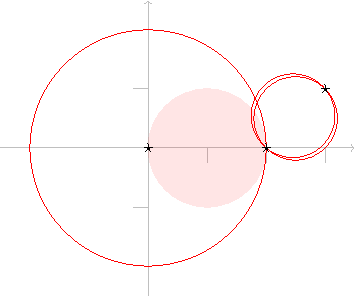
\includegraphics[width=.3\textwidth]{img/samples.pdf}


\section*{Pradiniai duomenys}

Pirmoje eilutėje pateikti keturi sveikieji skaičiai:
žvaigždžių, kurias astronomas nori stebėti, skaičius $k$,
šiąnakt danguje esančių žvaigždžių skaičius~$n$, 
teleskopo nukreipimo kaina~$s$ ir
teleskopo konstravimo kaina~$t$.
Toliau pateikta $n$ eilučių: $i$-ojoje eilutėje pateikiami du sveikieji skaičiai $x_i$ ir $y_i$ -- 
$i$-osios žvaigždės koordinatės.

\section*{Rezultatas}

Išveskite vieną realųjį skaičių: mažiausią kronų sumą, kurią teks astronomui išleisti.

\section*{Ribojimai ir vertinimas}

Visada galios šie ribojimai:
\begin{enumerate}
\item $1\leq k\leq n\leq 700$. % constraint:kn
\item $x_i, y_i\in \{-10^9,\ldots, 10^9\}$ kiekvienam $i\in\{1,\ldots,n\}$. % constraint:xy
\item $s,t\in \{0,\ldots, 10^9\}$. % constraint:st
\item Išvestis laikoma teisinga, jeigu jos ir teisingo atsakymo
santykinė arba absoliutinė paklaida yra ne didesnė nei $\epsilon = 10^{-6}$.
\end{enumerate}

Sprendimas bus testuojamas su keliomis testų grupėmis, kurių kiekviena verta tam tikro skaičiaus taškų.
Kiekviena testų grupė sudaryta iš įvairių testų.
Testų grupės taškai skiriami tik išsprendus visus grupės testus.
Galutinis taškų skaičius lygus daugiausiai surinkusio sprendimo taškų skaičiui.

\medskip
\noindent
\begin{tabular}{lll}
  Grupė & Taškai & Papildomi ribojimai\\\hline
  $1$ & $8$ &  $t\leq s$\\
  $2$ & $9$ & $n\le 50$ ir $s=0$\\
  $3$ & $18$ & $s=0$\\
  $4$ & $13$ & $n\leq 50$\\
  $5$ & $14$ & $n\leq 350$\\
  $6$ & $15$ & $\epsilon = 1/10$\\
  $7$ & $23$ & \emph{nėra}\\
\end{tabular}
